%% ReqWiki Documentation
%%
%% Copyright (C) 2012, 2013 Semantic Software Lab, http://www.semanticsoftware.info
%%
%% ReqWiki is free software: you can
%% redistribute and/or modify it under the terms of the GNU Affero General
%% Public License as published by the Free Software Foundation, either
%% version 3 of the License, or (at your option) any later version.
%% 
%% This program is distributed in the hope that it will be useful,
%% but WITHOUT ANY WARRANTY; without even the implied warranty of
%% MERCHANTABILITY or FITNESS FOR A PARTICULAR PURPOSE.  See the
%% GNU Affero General Public License for more details.
%% 
%% You should have received a copy of the GNU Affero General Public License
%% along with this program.  If not, see <http://www.gnu.org/licenses/>.
%%

\documentclass[10pt,twoside,openany,bibtotoc,liststotoc]{scrbook}
\usepackage{microtype}
\usepackage{bookman}
\usepackage{color}
\usepackage{url}
\usepackage{rotating}
\usepackage{listings}
\usepackage{booktabs}
\usepackage{amsmath}
\usepackage{hyperref}
\usepackage{xspace}
\usepackage{setspace}
\usepackage{verbatim}
%\usepackage{html}
\usepackage[round, sort]{natbib}

%% package options
% KOMA-Script
\typearea{12}
%%%%%%%%%%%%%%%%%%%%%%%%%%%%%%%%%%%%%%%%%%%%%%%%%%%%%%%%%%%%
%
%  Adding lines above and below the chapter head
%
 
% 1st get a new command
\newcommand*{\ORIGchapterheadstartvskip}{}%
% 2nd save the original definition to the new command
\let\ORIGchapterheadstartvskip=\chapterheadstartvskip
% 3rd redefine the command using the saved original command
\renewcommand*{\chapterheadstartvskip}{%
  \ORIGchapterheadstartvskip
  {%
    \setlength{\parskip}{0pt}%
    \noindent\rule[.3\baselineskip]{\linewidth}{1pt}\par
  }%
}
 
% see above
\newcommand*{\ORIGchapterheadendvskip}{}%
\let\ORIGchapterheadendvskip=\chapterheadendvskip
\renewcommand*{\chapterheadendvskip}{%
  {%
    \setlength{\parskip}{0pt}%
    \noindent\rule[.3\baselineskip]{\linewidth}{1pt}\par
  }%
  \ORIGchapterheadendvskip
}
%
%  End of chapter head change
%
%%%%%%%%%%%%%%%%%%%%%%%%%%%%%%%%%%%%%%%%%%%%%%%%%%%%%%%%%%%%

%% floats
\setcounter{topnumber}{2}
\setcounter{bottomnumber}{1}
\renewcommand{\floatpagefraction}{0.9}
\renewcommand{\topfraction}{0.9}
\renewcommand{\bottomfraction}{0.9}
\renewcommand{\textfraction}{0.1}

%% color definitions
\definecolor{darkred}{rgb}{0.5,0.0,0.0}
\definecolor{darkgreen}{rgb}{0.0,0.4,0.0}
\definecolor{darkblue}{rgb}{0.0,0.0,0.5}
\definecolor{gray}{gray}{0.8}
\addtokomafont{sectioning}{\color{blue}}

%% listing
\lstloadlanguages{Lisp,Java,Make,Ant}
\lstset{language=XML,
        basicstyle=\footnotesize\sffamily, %\ttfamily,
        keywordstyle=\color[rgb]{0.5,0,0.33203125}\bfseries,
        frame=shadowbox,
        rulesepcolor=\color{gray},
        commentstyle=\color[rgb]{0.24609375,0.5,0.37109375}, % commentstyle=\color{blue}\textit,
        extendedchars=true,
        showstringspaces=false,
        breaklines=true,
        breakatwhitespace=false,
        showlines=true,
        backgroundcolor=\color{white},
        numberstyle=\scriptsize,
        stepnumber=1,
        numbersep=5pt,
        numbers=left,
        stringstyle=\color[rgb]{0.1640625,0,1}\ttfamily}
%% url
\urlstyle{same}

%% hyperref
\hypersetup{
  backref=true,
  colorlinks=true,
  citecolor=darkgreen,
  linkcolor=darkred,
  urlcolor=darkblue,
  filecolor=red,
  letterpaper=false,
  bookmarks=true,
  bookmarksopen=true,
  pdfpagemode=UseOutlines,
  pdftitle={Semantic Assistants Documentation}, 
  pdfauthor={Semantic Software Lab}
}

\newcommand{\blankline}{\vspace{5mm}}

%\begin{comment}
%% miscellaneous macros
\newcommand{\sfcap}[1]{\strut\vspace*{-1mm}{\footnotesize\textsf{#1}}}
\newcommand{\filetilde}{\char126$\!\!$}
\newcommand{\argmax}{\mathop{\mathrm{argmax}}}
\newcommand{\sa}{Semantic Assistants\xspace}

\title{ReqWiki: A Semantic System for
Collaborative Software Requirements Engineering\bigskip\\
\Large Guide for Users and Developers}
\author{Ren\'{e} Witte\\
Bahar Sateli\\
Elian Angius\\
Srinivasan Rajivelu
\medskip}
\date{Development Release\\
\today
}
\publishers{Semantic Software Lab\\
Concordia University\\
Montr\'{e}al, Canada\\
{\large\url{http://www.semanticsoftware.info}}
}

\onehalfspacing

\graphicspath{{./graphics/}}

\begin{document}
\frontmatter
\maketitle

% Table of Contents
\pdfbookmark{Contents}{2}\tableofcontents

\section*{About this document}
This document contains documentation for the \emph{ReqWiki} project. You can obtain the latest version from
\url{http://www.semanticsoftware.info/reqwiki}. The project resources are hosted on GitHub,
\url{https://github.com/SemanticSoftwareLab/ReqWiki}. 

\section*{Licenses}
The ReqWiki project is
published under the GNU Affero General Public License v3
(AGPL3).\footnote{AGPL3,
\url{http://www.gnu.org/licenses/agpl-3.0.html}}

\mainmatter
\chapter{Overview}
The requirements engineering phase within a software project is a heavily knowledge-driven, collaborative process that typically involves the analysis and creation of a large number of textual artifacts. We know that requirements engineering has a large impact on the success of a project, yet sophisticated tool support, especially for small to mid-size enterprises, is still lacking. 

\blankline
Wikis, as an affordable and lightweight documentation and distributed collaboration platform, have demonstrated their capabilities in distributed requirements elicitation and documentation. While the integrity of software requirements specifications (SRS) documents inside a wiki can be enforced through the use of templates and wiki bots on a syntactic level, semantic SRS defects, such as ambiguity or inconsistency, require human revision. To this end, Natural Language Processing (NLP) techniques have been proposed as a means to (semi-)automatically improve requirements specifications, but so far have not been widely adopted. 

\blankline
In ReqWiki~[\cite{reqwiki2012}], we allows users to employ various state-of-the-art techniques from the NLP and Semantic Computing domains to improve the quality of SRS documents contained in a wiki platform, through using the NLP-provided guidance tips, as well as automatically detecting SRS defects.

\blankline
The core of ReqWiki is a MediaWiki\footnote{MediaWiki, \url{http://www.mediawiki.org}} engine, which provides a collaborative environment for SRS development. However, unadorned wikis can not fulfil all requirements, such as consistency management, semantic support, and natural language processing in the context of RE. For this, we added two substantial features to the wiki engine underlying ReqWiki, described in this user guide: a semantic data model and NLP web services.

\blankline
The rest of the this document is structured as follows: In Chapter~\ref{chap:feats} we present the ReqWiki features and how the wiki has been pre-filled with templates corresponding to the Unified Process methodology~[\cite{up}]. In Chapter~\ref{chap:install} we will guide you step-by-step on how to install ReqWiki. %Finally, development notes on how to customize the ReqWiki for your needs is described in Chapter~\ref{chap:develop}. 

\chapter{Features}
\label{chap:feats}
Based entirely on open source and open standards, ReqWiki is powered by MediaWiki - the powerful engine behind Wikipedia - and uses the Semantic MediaWiki extension to provide a technical platform with semantic support. The pre-defined semantic forms and templates in ReqWiki help users in creating various artifacts, while at the same time automatically creating the required semantic metadata. Figure~\ref{fig:reqwiki_ui} shows the user interface of ReqWiki.

\begin{figure}[h!]
  \centering
  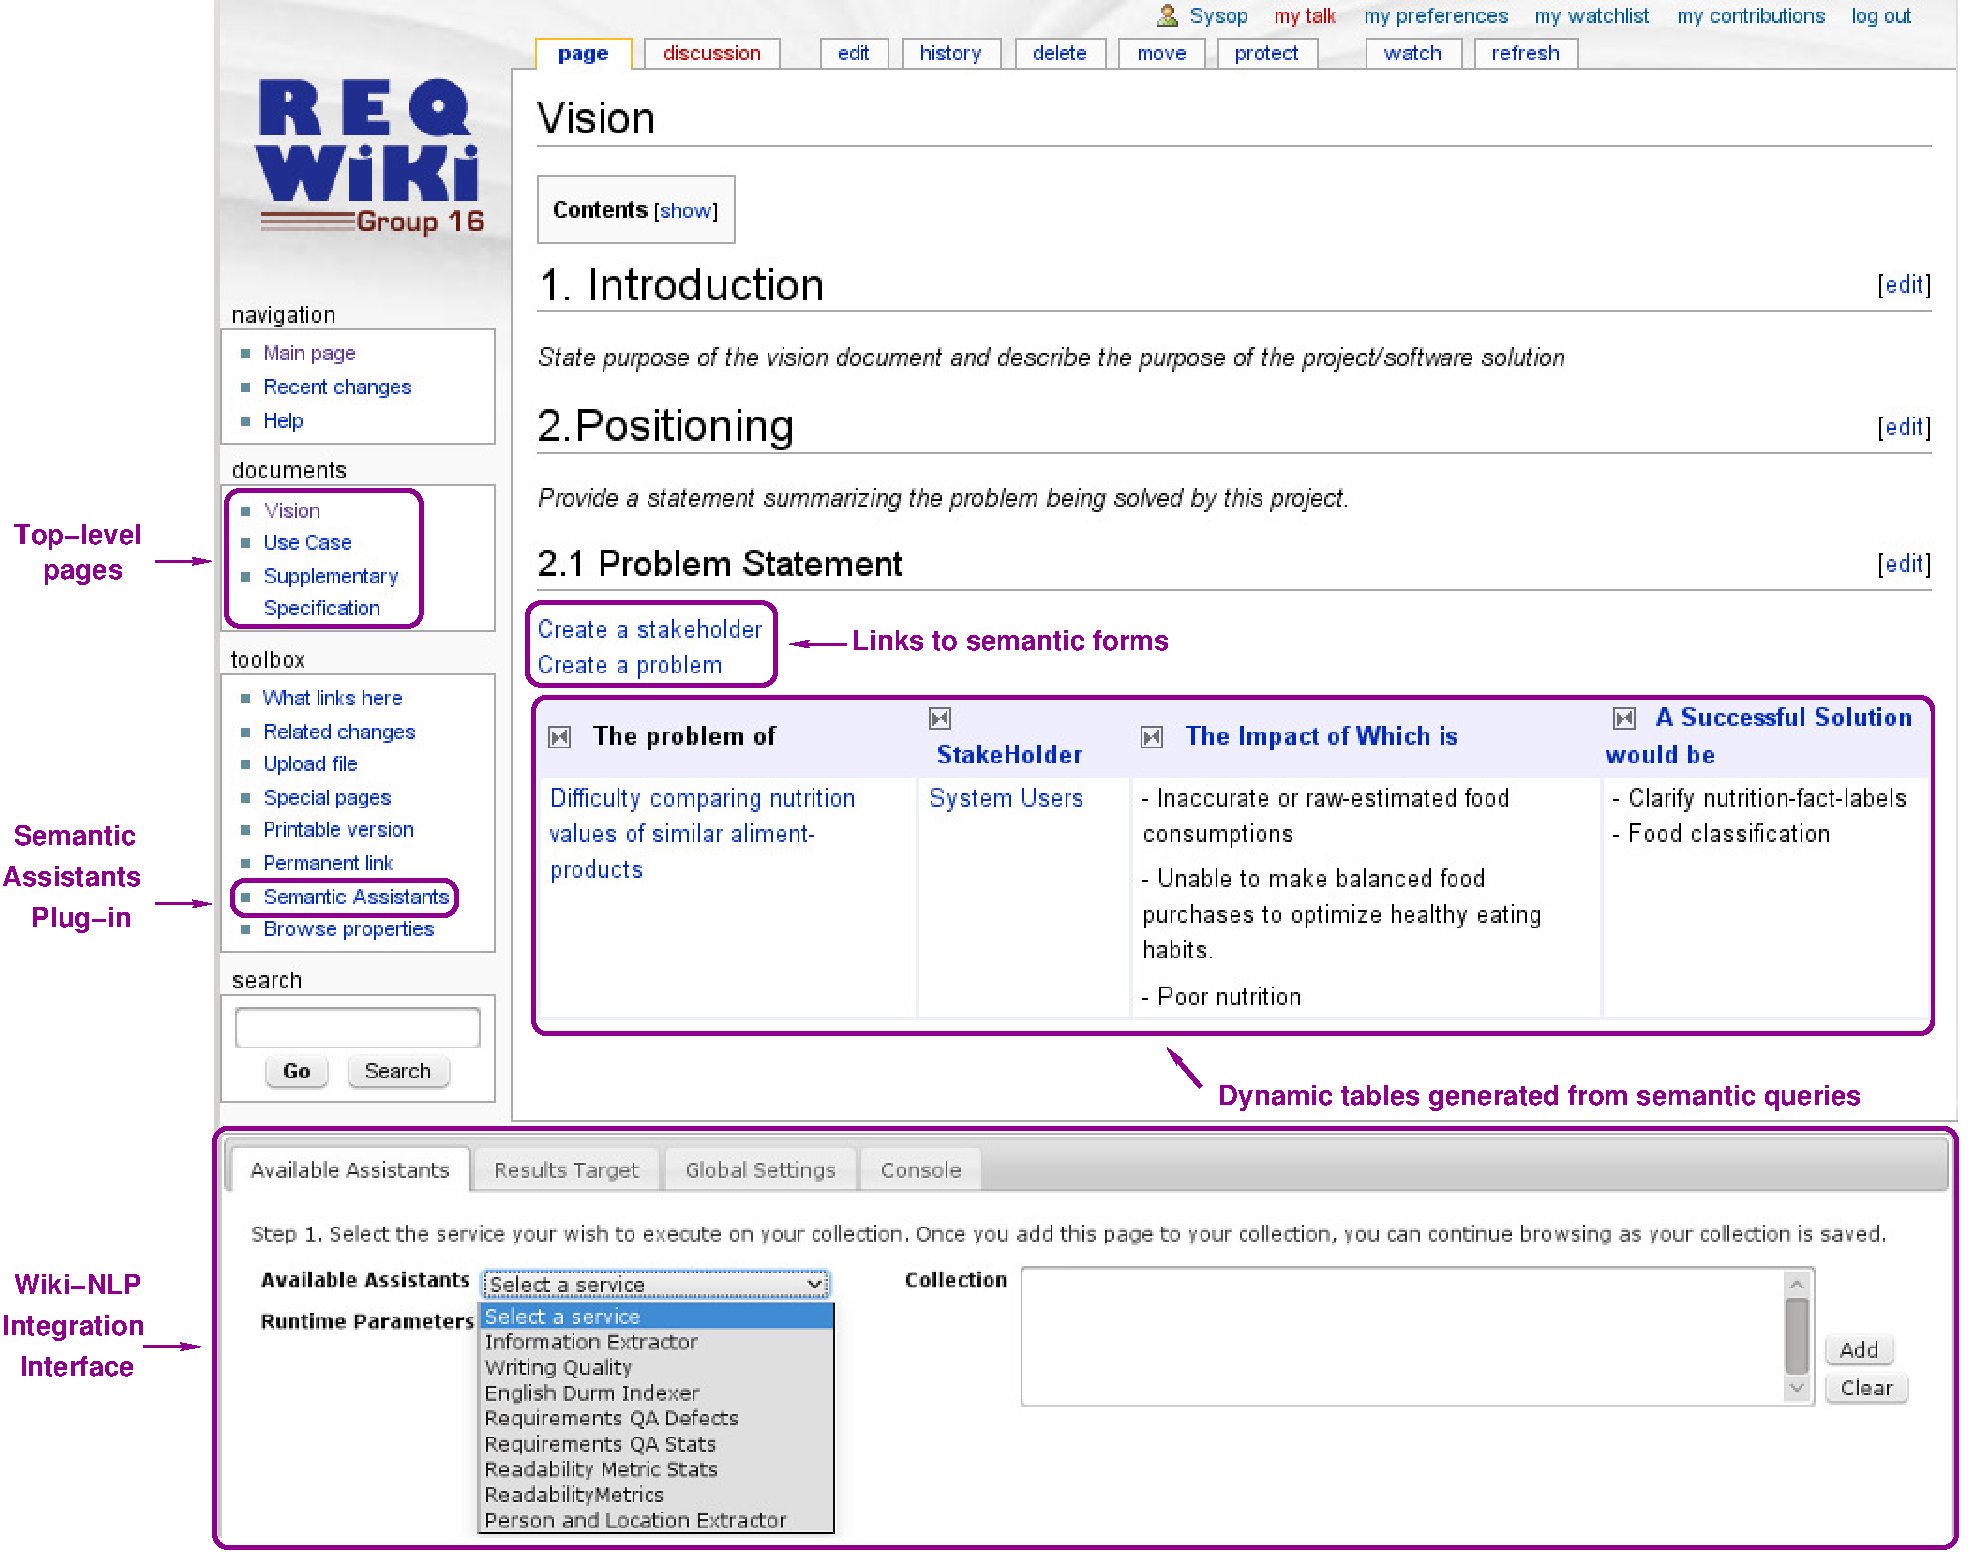
\includegraphics[width=\textwidth]{reqwiki}
  \caption{ReqWiki User Interface}
  \label{fig:reqwiki_ui}
\end{figure}

ReqWiki makes use of pre-defined templates to allow its users author SRS documents in a uniformed manner based on the UP methodology. The templates in ReqWiki (see Chapter \ref{chap:install}) conform to the UP methodology and its artifacts, such as vision document, use case document and applicable supplementary specifications. However, by using the same approach, other software development methodology artifacts can be easily added to the ReqWiki system. 

\section{Top-Level Documents}
ReqWiki features three top-level wiki pages that are considered the entry points to the SRS documentation platform and are designed to guide stakeholders through the RE process. For each top-level page, a corresponding ``talk'' page -- provided by the MediaWiki engine -- is also available for users to discuss contradictory ideas and leave notes for other stakeholders. The top-level pages are as follows:

%\begin{itemize}\itemsep-0.5em 
\begin{itemize}
\item a \textbf{Vision} page to define the product position, stakeholders, assumptions, dependencies, needs and features,
\item a \textbf{Use Case} page to define actors, goals and use cases,
\item a \textbf{Supplementary Specification} page to define functional and non-functional requirements, standards, legal notes, test cases and traceability links.
\end{itemize}

Each of these top-level pages is divided into multiple sections. Users can manually edit the static sections content, such as the introduction to the SRS document. The dynamic sections, on the other hand, are populated by the pre-defined queries embedded in the page markup every time the page is requested by a user. This way, it is ensured that the top-level pages are always presenting the latest state of the ReqWiki content.  In addition, at the bottom of all of three top-level pages, a list of user-defined terms is automatically generated and presented as a glossary to aid users in reflecting about the correct usage of the terms. The presence of this feature in ReqWiki helps to establish a common language among stakeholders and promotes consistency.

\section{Semantic Model}
In ReqWiki, to ensure consistency and compliance with a standard methodology, both within and between requirements artifacts, we formally model their concepts and relationships in a web ontology language. Using the ReqWiki underlying semantic wiki engine, we connect textual descriptions of artifacts with formal ontologies, providing further semantic reasoning and querying capabilities within the wiki environment. Our ReqWiki ontology defines the main concepts in the Unified Process and Use Case methodology for requirements engineering.  This ontology provides for the means to semantically describe concepts stored in the Wiki (e.g., actors, goals, use cases, test cases, features) and relate them with each other. For example, we can now formally establish the relations between a Use Case and its Actors.

Using this ontology, once the wiki content is enriched with semantic metadata, we are able to semantically query the ReqWiki content, e.g., to retrieve a list of all the actors in a wiki. In addition, reasoning capabilities can be added to the system to automatically detect inconsistencies and conflicts between entities.

\begin{figure}[h]
  \centering
  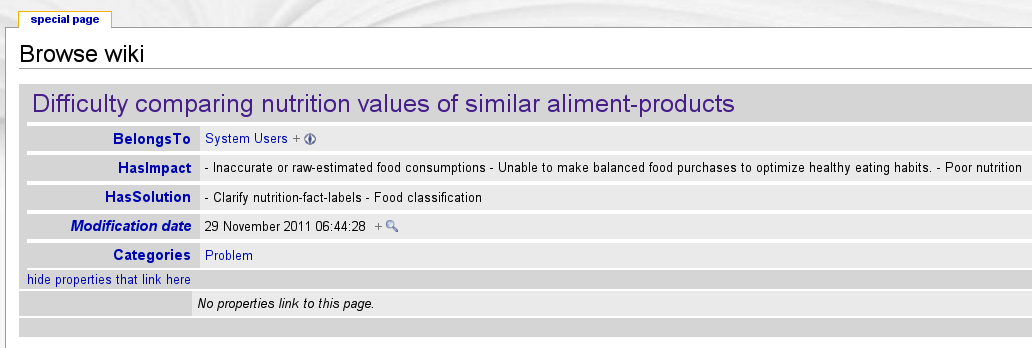
\includegraphics[width=0.8\textwidth]{reqwiki-rdf}
  \caption{Embedded RDF data associated with a ReqWiki entity)}
  \label{fig:form-rdf}
\end{figure}

\section{Semantic Forms}
Every entity in ReqWiki, like a use case description, is uniquely identified by a URI in the system and can be retrieved via its title or the full text search feature that the MediaWiki engine offers. Users can start defining entities like actors or goals, by clicking on the provided links in the top-level pages. For example, in the \emph{Use Case} page, a user can define a new use case description by clicking on the ``Create a use case'' link. The link takes the user to the corresponding \emph{semantic form} to define a use case attributes, such as actors, main success scenario, etc. These semantic forms are provided by the \emph{Semantic Form} extension installed on the ReqWiki engine and allow users to use user-friendly forms rather than directly dealing with wiki markup. Furthermore, the fields of each semantic form is related to a concept inside the ReqWiki semantic model, thus helps to simultaneously enrich the user provided data with semantic metadata. 

\begin{figure}[!ht]
  \centering
  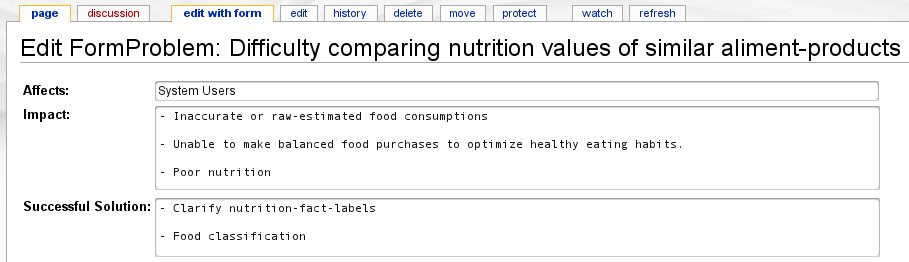
\includegraphics[width=0.8\textwidth]{reqwiki-forms}\\
  \caption{A ReqWiki Semantic Form}
  \label{fig:form}
\end{figure}

Once the user saves the form, a new page with the use case description is created in the wiki and the user input data embedded in the pre-defined ReqWiki template for a use case. Since the new page is implicitly annotated with semantic metadata, when the user navigates back to the top-level \emph{Use Case} page, he sees the new use case in a table that is generated by the in-line query embedded in the page, such as the one shown in Figure~\ref{fig:reqwiki_ui} (bottom).



\section{Automatic Traceability}

Motivated by maintainability and liability project factors,
\emph{traceability} is the degree to which various software artifacts in a
developing system are interrelated with each other.  In a collaborative and volatile environment such as RE, traceability ensures the rationale for all artifacts are properly accounted for towards building ``the right product''.  Manually creating and updating these links, for example, with cross-references between documents, is highly time-consuming and error prone.  Additionally, it must be possible to reference requirements artifacts from those produced in subsequent phases, such as design and code.

\blankline
Relying on the populated ontology, ReqWiki supports the automatic creation of three forms of traceability links: semantic links inside the wiki, query-based links, and revision links.


\begin{itemize}

\item For the first type, semantic concepts defined in wiki pages are presented as hyperlinks, so that users can navigate to and retrieve their corresponding content. When defining these semantic concepts, the forms themselves already constrain field input to non-empty existing ontology instances of the expected field type. Thus, this form of traceability enforces link correctness and simplifies verification and validation phases, since dead links and unlinkable artifacts are detectable.

\item For the second type, using the same semantic metadata in our ontology, we can insert in-line queries in top-level pages to create dynamic tables from the ontological meta-data. Figure~\ref{fig:traceability} shows the Need-Feature table dynamically generated from a SMW in-line query.

\begin{figure}[h!]
\centering
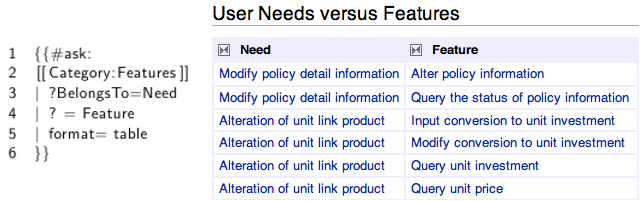
\includegraphics[width=0.8\textwidth]{traceability.png}
\caption{Embedded SMW query and resulting Feature-Need Table}
\label{fig:traceability}
\end{figure}

\item A third form of traceability available in the ReqWiki is revision control capabilities to when pages get changed. This not only indicates which author changed what content at which times, but also allows reverting to previous revisions in case of erroneous modifications.

\end{itemize}

\section{NLP Services}
The second major component of our ReqWiki system is the idea of semantic NLP \emph{assistants} that support users in developing the requirements specification. Our goal is to offer these analysis capabilities directly within the wiki, to avoid forcing users to switch to a different text analysis application. This is achieved through our Wiki-NLP integration (See Chapter~\ref{chap:develop}) that allows to setup an installation with custom NLP services, e.g., for domain-specific analysis pipelines or custom (company/organization-specific) quality rules. The integration is based on our \sa framework, which can broker any deployed NLP pipeline as a standard web service~[\cite{aswc08}]. Within the current version of ReqWiki, we have made a number of both general and requirements-specific NLP services available to ReqWiki users:

\begin{description}
\item[Writing Quality Assessment] is a service that integrates the After The Deadline~[\cite{Mudge10}] tool and helps ReqWiki users find spelling and grammatical mistakes and provides suggestions for improvements, where possible.

\item[Readability Metrics] is a service that provides an overall readability score of the content that users have produced, indicating how hard to read their text is for other stakeholders. This service provides the users with an overall readability score of the wiki content. The result score indicates how hard to read and comprehend the artifacts are for other stakeholders.
%It also can detect passive voice defects in wiki content.%It also can be used to trace the readability over time~\cite{1294952}.

\item[Requirements Quality Assurance] is a service developed based on the NASA requirements quality metrics~[\cite{Laplante09}] that detects SRS defects like \emph{Options, Directives} or \emph{Weak Phrases} in a document. By using this service, users have the chance to automatically find these defects in their specifications and correct them, resulting in a higher quality SRS document.

\item[Document Indexer] creates a back-of-the-book style index of the wiki content and stores it in the wiki as a page. This service builds on MuNPEx\footnote{Multi-Lingual Noun Phrase Extractor \url{http://www.semanticsoftware.info/munpex}}, an open-source tool that groups words into noun phrases, to generated an inverted index, with entries automatically linked to wiki pages.  Users can compare the result of this service to the glossary section of the SRS documents to check its completeness.

\item[Information Extractor] automatically extracts named entities, such as persons, organizations or locations, from wiki pages, based on the ANNIE system~[\cite{cun11}]. This service is especially useful in analysing existing domain documents during the requirements analysis phase.
\end{description}

These NLP pipelines can be executed on the ReqWiki content using the Wiki-NLP user interface shown in Figure~\ref{fig:reqwiki_sa}. Users can ask for this interface by clicking on the ``\sa'' link inside the wiki navigational menu (Figure~\ref{fig:reqwiki_sa} - left). The NLP interface allows users to see ``Available Assistants'' in the \sa server to help them with various NLP analyses. Hovering over each item in the list shows a brief description of what each service does. Once the user selects a service, he can then gather a so-called ``collection'' of wiki pages for analysis using the ``Add'' button.

\begin{figure}[h!]
\centering
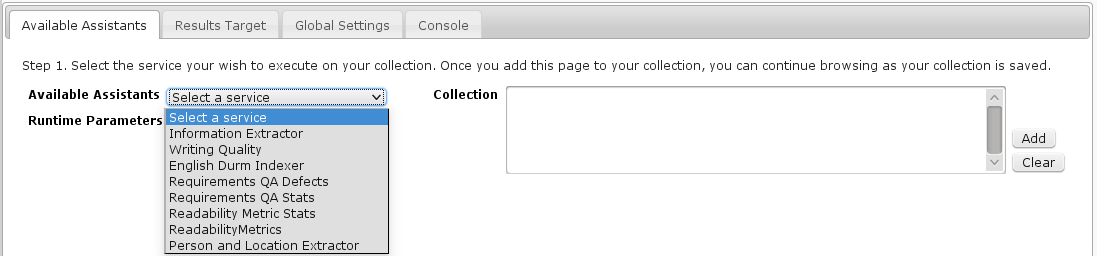
\includegraphics[width=\textwidth]{reqwiki-sa}
\caption{NLP services invocation interface in ReqWiki}
\label{fig:reqwiki_sa}
\end{figure}

\blankline
Next step is for users to specify where they would like the NLP analysis results be written to. The current options available the ``Target Options'' are:

\begin{description}
\item [``Same Page''], i.e., the results will be written in the same page as the resource. If the user has multiple pages in the collection, each results will be written into its corresponding source page. The current options for this item are the wiki page's main ``body'', or its associated ``talk''\footnote{In some MediaWiki skins, a talk page is also known as the ``discussion'' page.} section.
\item[``Another Page''], i.e., writing the results to a different page in the wiki. If the user has multiple pages in the collection, the results of all the wiki pages will be aggregated into one output and written into the specified wiki page. In order to precisely choose a destination for this option, users have to select a namespace from a list of available namespaces in the wiki and provide a unique page name. If the specified wiki page exists in the wiki, the results will be appended to the end of the page, otherwise a new wiki page will be automatically created.
\item[``Another Wiki''] i.e., writing the results of the analysis into a different wiki than the source, provided that its engine is supported by the integration. Needless to say, users must provide the integration with (1) the address of the destination wiki, (2) its underlying wiki engine and version, (3) a valid username and password, and (4) a valid page name. Similar to the previous option, the results of the analysis will be aggregated and made persistent in the destination wiki page.
\end{description}

A service execution request can then be made by clicking on the ``Run'' button in the second tab. The ``Console'' tab of the Wiki-NLP interface shows user-friendly logs of the NLP service execution and indicates where the results are written if the execution is successfully done.

Where applicable, users can dynamically change which \sa server they want their wiki to connect to. The ``Global Settings'' tab in the Wiki-NLP interface shown in Figure~\ref{fig:reqwiki_sa}, allows users to select a \sa server from a list of pre-defined addresses, as well as defining a custom end point. Once the user clicks the ``connect'' button, the selected server address is stored in the browser cookies and will take effect as soon as the user refreshes the browser.

\chapter{Installation}
\label{chap:install}
ReqWiki is an open source software released under APGL3 license and its resources can be downloaded freely from the Semantic Software Lab public repository on GitHub website accessible from \url{https://github.com/SemanticSoftwareLab/ReqWiki}.

\section{Downloading Resources from GitHub}
In order to download the ReqWiki resources from GitHub, there are two options:

\begin{enumerate}
\item \textbf{Downloading a .zip file. } All the ReqWiki resources can be downloaded a \texttt{.zip} file directly from the GitHub website. To do so, browse to \url{https://github.com/SemanticSoftwareLab/ReqWiki} on your web browser and click on the ``Zip'' button on top of the page. Then, save and unzip the file to your local workstation.
\item \textbf{Cloning the repository. } You can also acquire a read-only version of the ReqWiki resources from a command line terminal of your choice. Note that you need to have Git\footnote{Git, \url{http://git-scm.com/}} installed on your system. Provided, browse to a desired directory in your local workstation and type the following line in your command line terminal:
\blankline

\centering
\begin{lstlisting}[language=xml,numbers=left,xleftmargin=4mm,columns=flexible]
git clone https://github.com/SemanticSoftwareLab/ReqWiki.git
\end{lstlisting}
\end{enumerate}

\section{MediaWiki Installation}
Once you have the resources, you need to install a MediaWiki instance on a web server. ReqWiki required MediaWiki version 1.16 to function properly. Installation details of MediaWiki instances can be found on the MediaWiki website\footnote{MediaWiki Installation, \url{http://www.mediawiki.org/wiki/Help:Installation}}.

\section{MediaWiki Extensions}
In addition the MediaWiki default installation, ReqWiki requires a number of extensions to be installed on the wiki.

\subsection{Semantic MediaWiki}
To provide semantic enrichment and query of the wiki content, ReqWiki requires Semantic MediaWiki extension version 1.5 or higher. First download the SMW extension from the Semantic MediaWiki website\footnote{SMW Website, \url{http://www.semantic-mediawiki.org/wiki/Semantic\_MediaWiki}}. Unzip and copy the extension to the \url{extensions} folder in the root of your wiki installation. Next, paste the following lines at the end of the \texttt{LocalProperties.php} file in the root of your wiki installation.

\begin{center}
\begin{lstlisting}[language=xml,numbers=left,xleftmargin=4mm,columns=flexible]
include_once("$IP/extensions/SemanticMediaWiki/SemanticMediaWiki.php");
enableSemantics('localhost');
\end{lstlisting}
\end{center}

These two lines \emph{install} the SMW extension on your wiki, but we still need to initialize the SMW tables in the wiki database. To do so, browse the special pages of your wiki and click on the ``Admin Admin functions for Semantic MediaWiki'' link under the ``Semantic MediaWiki'' category. On the next page click on the ``Initialise or upgrade tables'' button to start the database initialization process.

\subsection{Semantic Forms}
Similar to the SMW extension, ReqWiki requires the Semantic Forms extension to be installed on its MediaWiki engine. First download the extension from the MediaWiki website\footnote{Semantic Form extension, \url{http://www.mediawiki.org/wiki/Extension:Semantic_Forms}}. Then copy the file to the \url{extensions} folder of your wiki and add the following line to the end of the \texttt{LocalProperties.php} file in the root of your wiki installation.

\begin{center}
\begin{lstlisting}[language=xml,numbers=left,xleftmargin=4mm,columns=flexible]
include_once("$IP/extensions/SemanticForms/SemanticForms.php");
\end{lstlisting}
\end{center}

\subsection{Semantic Assistants}
One last extension to install on your MediaWiki instance in the \sa extensions. This extension provides the Wiki-NLP user interface shown above in the wiki. To do so, copy the \sa extension inside the \url{extension} folder in your ReqWiki check-out over to the \url{extensions} folder of your MediaWiki installation. Finally, add the following line to the end of the \texttt{LocalProperties.php} file of your wiki.

\begin{center}
\begin{lstlisting}[language=xml,numbers=left,xleftmargin=4mm,columns=flexible]
include_once("$IP/extensions/SemanticAssistants/SemanticAssistants.php");
\end{lstlisting}
\end{center}

\subsection{ReqWiki Templates}
After installing the extensions, we need to install ReqWiki customized templates to pre-fill the wiki with top-level pages, forms and semantic properties pertaining to the wiki semantic model. In order to import the templates to your wiki, browse to the special pages of your wiki and click on the ``Import pages'' link under the ``Page tools'' category\footnote{In the default installation of MediaWiki, permission of importing pages to the wiki is limited to users with the ``admin'' role.}. From the ``\texttt{Import XML data}'' box click on the ``\texttt{Browse}'' button and upload the \url{ReqWiki_templates.xml} file located in the \url{templates} folder of your ReqWiki check-out, as shown in Figure~\ref{fig:wiki_template_import}.

\begin{figure}[h!]
\centering
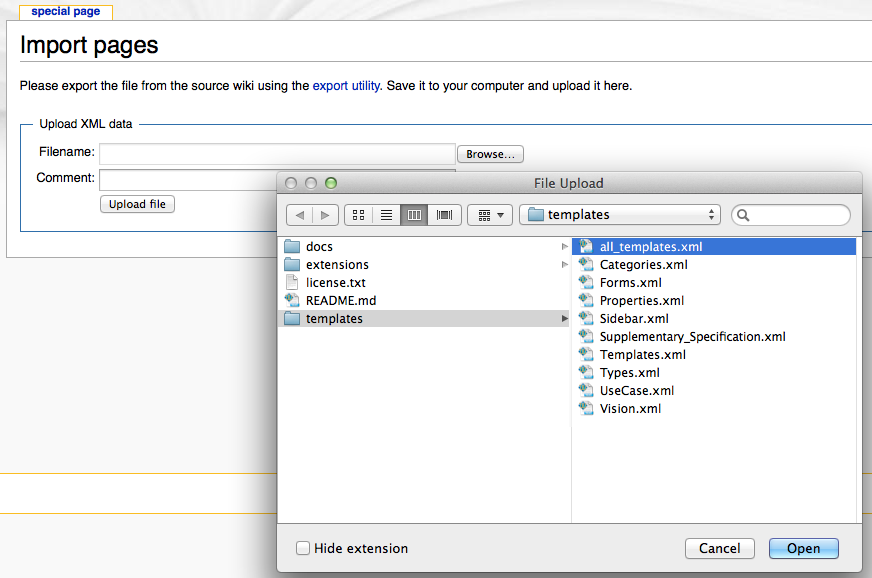
\includegraphics[width=\textwidth]{reqwiki_template_import.png}
\caption{Importing ReqWiki templates into MediaWiki engine}
\label{fig:wiki_template_import}
\end{figure}


\chapter{Development Notes}
\label{chap:develop}
Although the templates in ReqWiki have been designed to conform to the UP methodology, by using the same approach, other software development methodology artifacts can be easily added to the ReqWiki system. Also, since ReqWiki is empowered by an open service-oriented architecture, additional NLP services can be added to ReqWiki with little effort. In this chapter, we describe the system architecture behind the ReqWiki and how new NLP services can be added to the architecture.

\section{System Architecture}
The text mining capabilities in ReqWiki are provided by a novel integration of NLP within wiki systems. The Wiki-NLP integration~[\cite{wikinlp2012}] is a cohesive architecture that provides a seamless integration of NLP techniques within wiki environments. The ReqWiki architecture, shown in Figure~\ref{fig:wikinlp_arch}, is mainly composed on two components; A server-side component delegates the NLP services requests to the \sa framework -- an open source framework that publishes concrete NLP pipelines as standard web services~[\cite{aswc08}]. And a client-side, light-weight plug-in that needs to be installed on the wiki engine. The communication between the two end points are performed over standard HTTP protocols and is realized through custom JavaScript code that is injected into the user's browser.

\begin{figure}[h!]
\centering
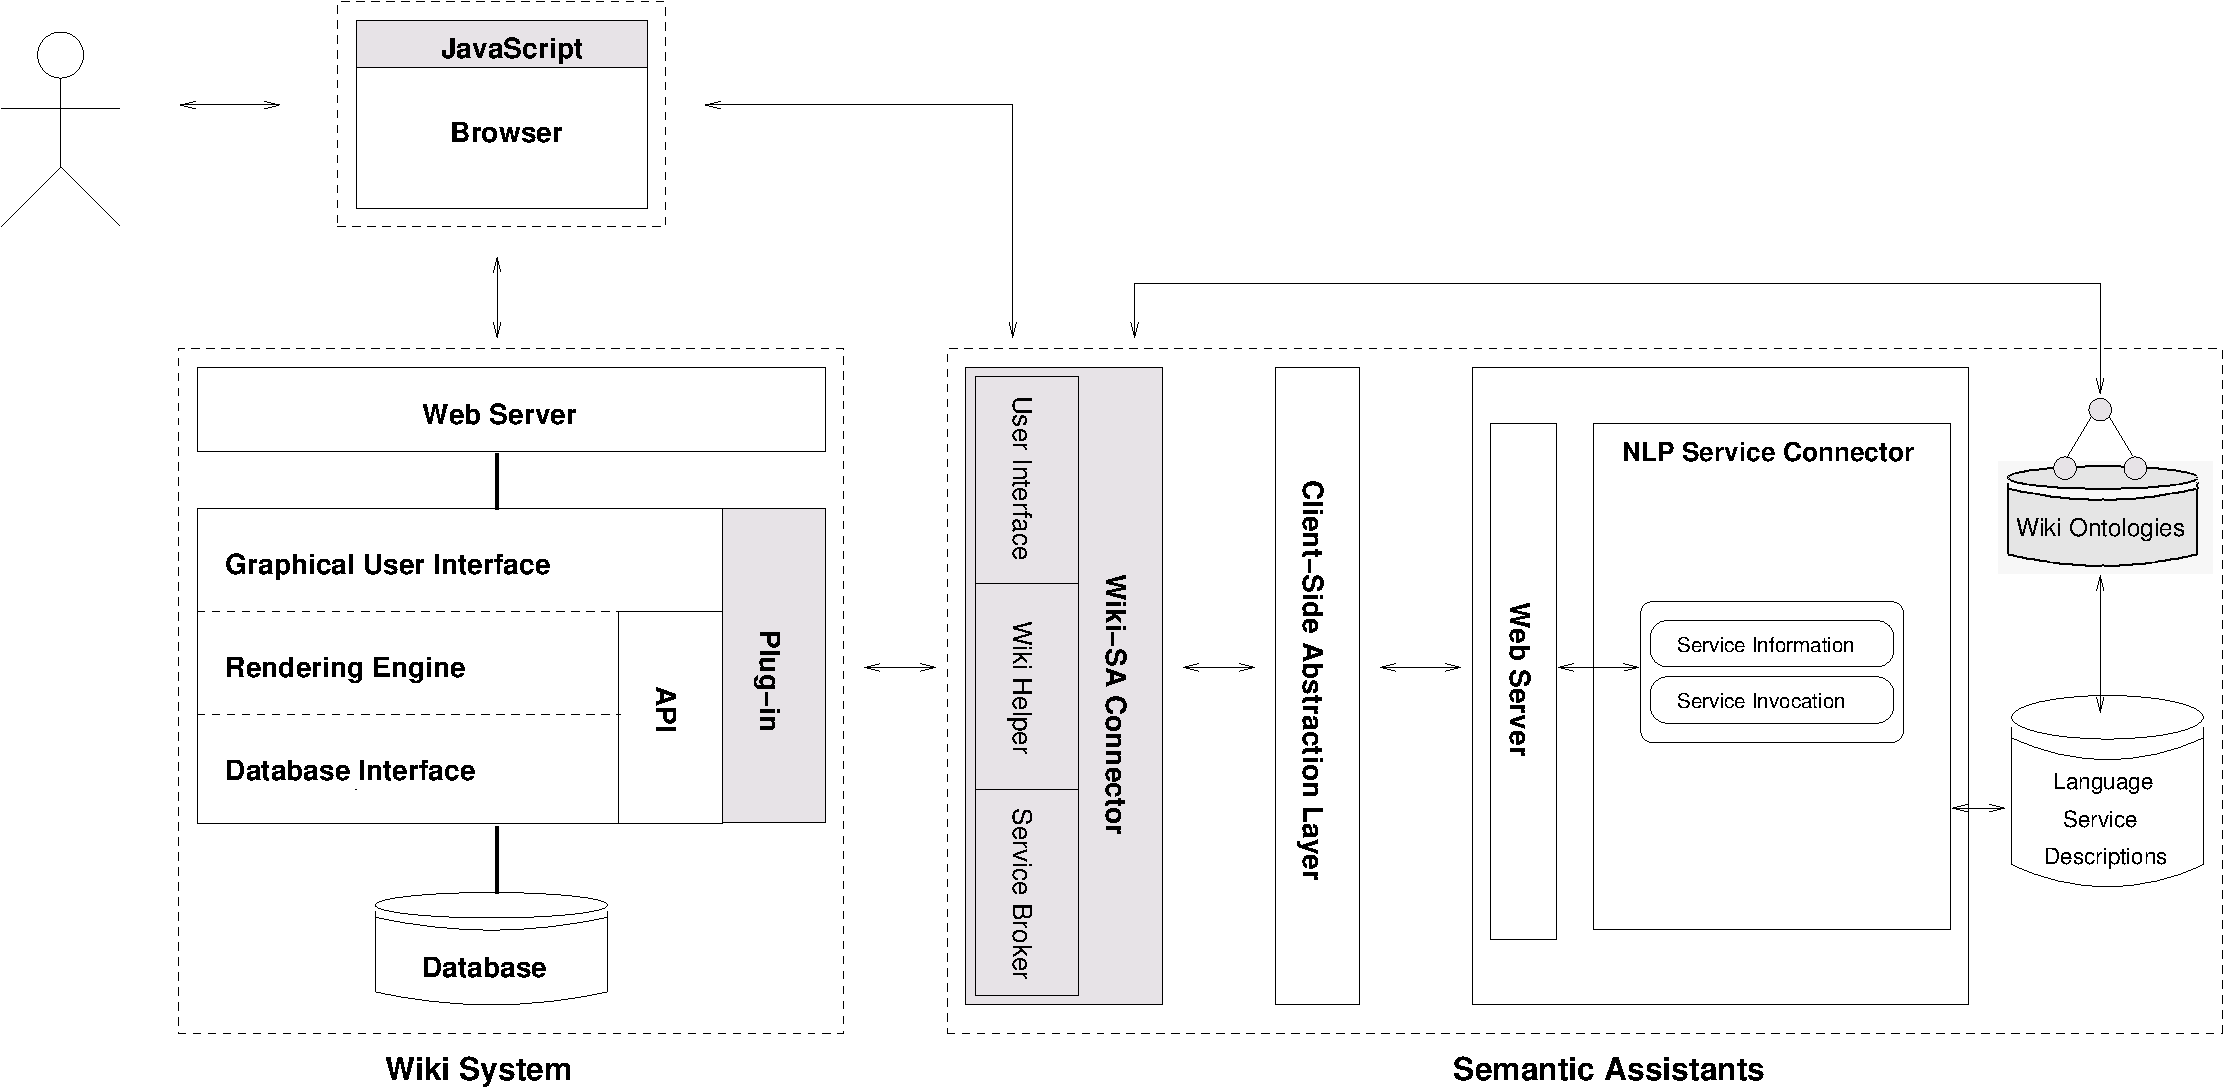
\includegraphics[width=0.79\textwidth]{wikinlp_arch}
\caption{Wiki-NLP integration architecture in ReqWiki}
\label{fig:wikinlp_arch}
\end{figure}

\section{Adding New NLP Services}
By default the ReqWiki NLP services are provided by a pre-defined \sa server configured in its architecture. If you would like to offer additional NLP services within your ReqWiki environment, you have to set up a \sa server with your custom NLP services deployed in it. To do so, please consult the \sa user guide\footnote{\sa, url{http://www.semanticsoftware.info/semantic-assistants}} on how to set up a custom \sa server.

Once the new server is up and running, you can configure your ReqWiki to connect to the your \sa server rather than its default one. You can do so through the NLP interface in the wiki. In the ``Global Settings'' tab, shown in Figure~\ref{fig:wikinlp_settings}, select the ``Custom Server'' option and fill in the host name and port number fields and click ``Add Server''. Then select the ``Pre-defined Servers'' option, choose your new server from the list and click on ``Connect''. The new changes will take effect next time you refresh your browser.

\begin{figure}[h!]
\centering
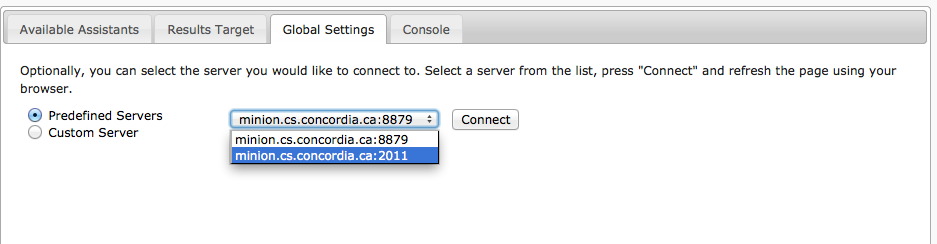
\includegraphics[width=\textwidth]{wikinlp_settings.png}
\caption{Wiki-NLP integration architecture in ReqWiki}
\label{fig:wikinlp_settings}
\end{figure}

\backmatter
%\appendix
\bibliographystyle{plainnat}
\bibliography{reqwiki_manual}

\end{document}
